\documentclass{standalone}

\usepackage[english]{babel}
\usepackage[linesnumbered, ruled, vlined]{algorithm2e}

\usepackage{caption}
\usepackage{listings, lstautogobble}
\lstset{
  autogobble=true,
  frame=single,
}

\lstdefinelanguage{coq}[Objective]{Caml}{
  morekeywords={Structure, Definition, Inductive, list, return},
  sensitive=true
}

\usepackage{ulem}
\usepackage{moresize}
\usepackage{anyfontsize}
\usepackage{pgfplots}
\pgfplotsset{compat=1.13}
\usepackage{tikz-timing}
\usepackage{tikz}

\usetikzlibrary{backgrounds}
\usetikzlibrary{positioning, calc, arrows, shapes, automata, petri, patterns}
\tikzset{every picture/.style={remember picture}}

\usepackage{xcolor}

\begin{document}

\tikzset{transition/.append style={fill=black!20, thick}}

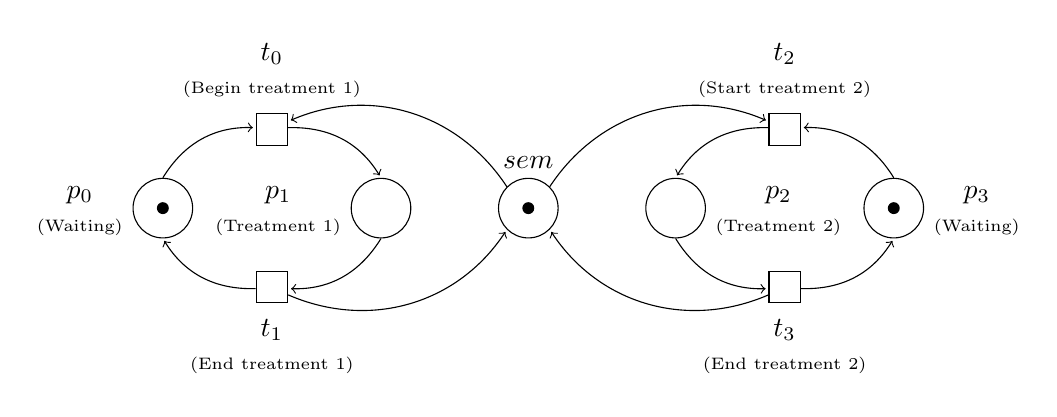
\begin{tikzpicture}

  %%%%%%%%%%% First process %%%%%%%%%%
  
  % Proc 1 works alone
  \node[place, tokens=1] (proc1wa) {};

  \node[anchor=east] at ($(proc1wa.west)$) {
    \begin{tabular}{@{}c@{}}
      $p_0$ \\
      \ssmall (Waiting) \\
    \end{tabular}
  };

  
  % Treatment 1
  \node[place] (treatment1) [right =20mm of proc1wa] {};

  \node[anchor=east] at ($(treatment1.west)$) {
    \begin{tabular}{@{}c@{}}
      $p_1$ \\
      \ssmall (Treatment 1) \\
    \end{tabular}
  };
  
  % Semaphor
  \node[place, tokens=1] (sem) [right =11mm of treatment1,
  label={above: $sem$}] {};

  %%%%%%%%%%>> transitions
  
  % Begin treatment 1
  \node[transition] (proc1eow) at ($(proc1wa)!0.5!(treatment1)+(0,1)$)
  [] {}
  edge[pre, bend right] (proc1wa.north)
  edge[pre, bend left=40] (sem.north west)
  edge[post, bend left] (treatment1.north);

  \node[anchor=south] at ($(proc1eow.north)$) {
    \begin{tabular}{@{}c@{}}
      $t_0$ \\
      \ssmall (Begin treatment 1) \\
    \end{tabular}
  };
  
  % End treatment 1
  \node[transition] (proc1eot) at ($(proc1wa)!0.5!(treatment1)-(0, 1)$)
   {}
  edge[pre, bend right] (treatment1.south)
  edge[post, bend right=40] (sem.south west)
  edge[post, bend left] (proc1wa.south);

  \node[anchor=north] at ($(proc1eot.south)$) {
    \begin{tabular}{@{}c@{}}
      $t_1$ \\
      \ssmall (End treatment 1) \\
    \end{tabular}
  };
  
  %%%%%%%%%%% Second process %%%%%%%%%%
  
  % Proc 2 works alone
  \node[place] (proc2wa) [right =11mm of sem] {};
  \node[anchor=west] at ($(proc2wa.east)$) {
    \begin{tabular}{@{}c@{}}
      $p_2$ \\
      \ssmall (Treatment 2) \\
    \end{tabular}
  };
  
  % Treatment 2
  \node[place, tokens=1] (treatment2) [right =20mm of proc2wa] {};
  \node[anchor=west] at ($(treatment2.east)$) {
    \begin{tabular}{@{}c@{}}
      $p_3$ \\
      \ssmall (Waiting) \\
    \end{tabular}
  };
  
  %%%%%%%%%%>> transitions
  
  % Begin treatment 2
  \node[transition] (proc2eow) at ($(proc2wa)!0.5!(treatment2)+(0,1)$) {}
  edge[post, bend right] (proc2wa.north)
  edge[pre, bend right=40] (sem.north east)
  edge[pre, bend left] (treatment2.north);

  \node[anchor=south] at ($(proc2eow.north)$) {
    \begin{tabular}{@{}c@{}}
      $t_2$ \\
      \ssmall (Start treatment 2) \\
    \end{tabular}
  };
  
  % End treatment 2
  \node[transition] (proc2eot) at ($(proc2wa)!0.5!(treatment2)-(0, 1)$)
  {}
  edge[post, bend right] (treatment2.south)
  edge[pre, bend left] (proc2wa.south)
  edge[post, bend left=40] (sem.south east); 

  \node[anchor=north] at ($(proc2eot.south)$) {
    \begin{tabular}{@{}c@{}}
      $t_3$ \\
      \ssmall (End treatment 2) \\
    \end{tabular}
  };
    
\end{tikzpicture}

\end{document}

%%% Local Variables:
%%% mode: latex
%%% TeX-master: t
%%% End:
